\subsection{Metaheurísticas aplicadas en las pruebas}
A continuación se mostrarán las metaheurísticas aplicadas en los experimentos, primero se explicarán los pasos realizados que se muestran en el diagrama de la figura \ref{fig:FLOWCHART2}, después se mostrará la funcionalidad de cada metaheurística programada para este experimento junto con la configuración de parámetros usados en el mismo.
\begin{figure}[hbtp]
   \centering
   \begin{tikzpicture}[node distance=1.6cm]

        \node (start) [startstop] 
		{
				Inicio
		};
        \node (in1) [io, below of=start, text width=5cm] 
		{
        	Recibe un problema de TSP
        };
        \node (pro1) [process, below of=in1, yshift=-0.1cm, text width=12cm] 
		{
        	Resolver el problema por el método de cuadrantes (solución original)
        };       
        \node (pro2) [process, below of=pro1, yshift=-0.1cm, text width=12cm] 
		{
        	Se aplicará una metaheurística (Recocido Simulado, Greedy o Genético) para mutar la solución original
        };    
        \node (in2) [io, below of=pro2, text width=5cm] 
		{
        	Se guardará el resultado obtenido
        };
        \node (pro3) [process, below of=in2, yshift=-0.1cm, text width=12cm] 
		{
        	 Se volverá a mutar la solución original cuantas veces se requiera 
        }; 
        \node (pro4) [process, below of=pro3, yshift=-0.1cm, text width=12cm] 
		{
           De los resultados obtenidos se clasificará el mejor, peor y promedio así mismo se comparará por problema cual fue el mejor de los 3
        }; 
        \node (pro5) [process, below of=pro4, yshift=-0.1cm, text width=12cm] 
		{
           Así mismo se harán experimentos saltándose el método de cuadrantes y se anotarán los resultados en una comparativa diferente
        }; 
        \node (Fin) [startstop, below of=pro5, yshift=-0.1cm,] 
		{
				Fin
		};
        
        \draw [arrow] (start) -- (in1);
        \draw [arrow] (in1) -- (pro1);
        \draw [arrow] (pro1) -- (pro2);
        \draw [arrow] (pro2) -- (in2);
        \draw [arrow] (in2) -- (pro3);
        \draw [arrow] (pro3) -- (pro4);
        \draw [arrow] (pro4) -- (pro5);
        \draw [arrow] (pro5) -- (Fin);
		
    \end{tikzpicture}       
    \caption{Diagrama de flujo del experimento de método de cuadrantes con metaheurísticas.}
    \label{fig:FLOWCHART2}
\end{figure} 
\clearpage \newpage

\subsubsection{Algoritmo de Recocido Simulado}
Aquí se aplicará lo aprendido en el código \ref{lst:recocidosimulado} donde usando un valor de aleatoriedad combinado con la diferencia de resultados obtenidos se irá viendo si el resultado (mejor o peor que el anterior) será el objetivo actual. En la tabla \ref{table:ConfiguracionRS.tsp} se describen las variables usadas y en el código \ref{lst:AlgoritmoRecocidoSimuladoPruebas} se muestra la implementación del algoritmo de Recocido simulado.  

% Please add the following required packages to your document preamble:
% \usepackage[table,xcdraw]{xcolor}
% If you use beamer only pass "xcolor=table" option, i.e. \documentclass[xcolor=table]{beamer}
\begin{table}[hbtp]
\centering
\caption{Configuración de las variables de recocido simulado durante las pruebas.}
\begin{tabular}{llr}
\hline
\rowcolor[HTML]{656565} 
\multicolumn{1}{c}{\cellcolor[HTML]{656565}{\color[HTML]{FFFFFF} \textbf{Nombre}}} & \multicolumn{1}{c}{\cellcolor[HTML]{656565}{\color[HTML]{FFFFFF} \textbf{Descripción}}}                                    & \multicolumn{1}{c}{\cellcolor[HTML]{656565}{\color[HTML]{FFFFFF} \textbf{Valor}}} \\ \hline
Ciclos                                                                             & Cantidad de veces en que se repetirá el proceso                                                                            & 10000                                                                             \\ \hline
Genes máximos                                                                      & \begin{tabular}[c]{@{}l@{}}La cantidad de genes que tendrá la especie durante \\ el proceso de búsqueda local\end{tabular} & 100                                                                               \\ \hline
Distancia gen mínimo                                                               & \begin{tabular}[c]{@{}l@{}}El número mínimo que tendrá en el intercambio de \\ posiciones\end{tabular}                     & 2                                                                                 \\ \hline
Distancia gen máximo                                                               & \begin{tabular}[c]{@{}l@{}}El número máximo que tendrá en el intercambio de \\ posiciones\end{tabular}                     & 5                                                                                 \\ \hline
Temperatura inicial                                                                & Al momento de capturarse se multiplica por $10^{-10}$                                        								& 600                                                                               \\ \hline
\end{tabular}

\label{table:ConfiguracionRS.tsp}
\end{table} 

\begin{lstlisting}[language=C++, caption=Algoritmo de recocido simulado aplicado en las pruebas, label=lst:AlgoritmoRecocidoSimuladoPruebas]
    Inicio
    
    Ciclos
    Genes máximos
    Distancia gen mínimo
    Distancia gen máximo
    Factor de temperatura
    
    Recibir una lista de puntos para trabajar convirtiéndose en la lista de puntos actual.
    MIENTRAS(NO se hayan cumplido la cantidad de Ciclos){
    	1.- Crear una nueva especie con una longitud igual a la cantidad de genes máximos.
    	2.- Los números que conformara la especie oscilara entre el número mínimo y máximo declarados anteriormente.
    	3.- Una vez declarada alterara la lista de puntos actual para obtener una lista nueva.
    	4.- Una vez alterada la lista de puntos actual con la nueva, en caso de obtener un mejor resultado 
    	SI(el resultado es mejor){
    		1.-esta lista es sustituida por la nueva.
    	}SINO{
    		1.-Aplicar formula de temperatura
    		SI(APLICA){
    		    1.-La especie, aunque ineficiente se convierte en la lista de puntos actual.
    		    2.-Se ajusta la temperatura.
    		}
    	}
    }
    
    Fin
\end{lstlisting}

\clearpage \newpage

\subsubsection{Algoritmo Greedy}
A diferencia del algoritmo de recocido simulado, el algoritmo Greedy (o voraz) es más directo, intenta sacar al azar una solución y verifica que éste sea el mejor, si lo es sustituye al original, sino lo es lo descarta y continua el proceso hasta que se cumpla el criterio de paro, que en este caso son el número de veces (o ciclos) que se repetirá el proceso. En la tabla \ref{table:ConfiguracionGR.tsp} se describen las variables usadas y en el código \ref{lst:AlgoritmoGreedyPruebas} muestra la implementación del algoritmo Greedy.

% Please add the following required packages to your document preamble:
% \usepackage[table,xcdraw]{xcolor}
% If you use beamer only pass "xcolor=table" option, i.e. \documentclass[xcolor=table]{beamer}
\begin{table}[hbtp]
\centering
\caption{Configuración de las variables de método greedy durante las pruebas.}
\begin{tabular}{llr}
\hline
\rowcolor[HTML]{656565} 
\multicolumn{1}{c}{\cellcolor[HTML]{656565}{\color[HTML]{FFFFFF} \textbf{Nombre}}} & \multicolumn{1}{c}{\cellcolor[HTML]{656565}{\color[HTML]{FFFFFF} \textbf{Descripción}}}                                    & \multicolumn{1}{c}{\cellcolor[HTML]{656565}{\color[HTML]{FFFFFF} \textbf{Valor}}} \\ \hline
Ciclos                                                                             & Cantidad de veces en que se repetirá el proceso.                                                                            & 10000                                                                             \\ \hline
Genes máximos                                                                      & \begin{tabular}[c]{@{}l@{}}La cantidad de genes que tendrá la especie durante \\ el proceso de búsqueda local.\end{tabular} & 100                                                                               \\ \hline
Distancia gen mínimo                                                               & \begin{tabular}[c]{@{}l@{}}El número mínimo que tendrá el intercambio de \\ posiciones.\end{tabular}                     & 2                                                                                 \\ \hline
Distancia gen máximo                                                               & \begin{tabular}[c]{@{}l@{}}El número máximo que tendrá el intercambio de \\ posiciones.\end{tabular}                     & 5                                                                                 \\ \hline
\end{tabular}
\label{table:ConfiguracionGR.tsp}
\end{table} 

\begin{lstlisting}[language=C++, caption=Algoritmo greedy aplicado en las pruebas, label=lst:AlgoritmoGreedyPruebas]
    Inicio
    
    Ciclos
    Genes máximos
    Distancia gen mínimo
    Distancia gen máximo
    
    Recibir una lista de puntos para trabajar convirtiéndose en la lista de puntos actual.
    MIENTRAS(NO se hayan cumplido la cantidad de Ciclos){
    	1.- Crear una nueva especie con una longitud igual a la cantidad de genes máximos
    	2.- Los números que conformará la especie oscilará entre el número mínimo y máximo declarados anteriormente
    	3.- Una vez declarada alterara la lista de puntos actual para obtener una lista nueva.
    	4.- Una vez alterada la lista de puntos actual con la nueva, en caso de obtener un mejor resultado esta lista es sustituida por la nueva
    }
    
    Fin
\end{lstlisting}

\clearpage \newpage

\subsubsection{Algoritmo Genético}
Por último el algoritmo genético en vez de modificar una solución candidata, utiliza una población de ellas donde soluciones con mejor resultado tendrá la prioridad para reproducirse, y durante varias generaciones los descendientes irán modificando el resultado original hasta que al final devuelva uno mejor. Entre los aspectos a destacar son el hecho de dividir los genes en dominantes y recesivos: los primeros jamás se modificarán y representan aquellos cambios que son capaces de mejorar el resultado y luego están los recesivos que estarán sujetos a una mutación devolviendo otro conjuntos de valores numéricos que pueden o no mejorar la solución. En la tabla \ref{table:ConfiguracionAG.tsp} se describen las variables usadas y en el código \ref{lst:AlgoritmoGeneticoPruebas} muestra la implementación del algoritmo genético.

% Please add the following required packages to your document preamble:
% \usepackage[table,xcdraw]{xcolor}
% If you use beamer only pass "xcolor=table" option, i.e. \documentclass[xcolor=table]{beamer}
\begin{table}[hbtp]
\centering
\caption{Configuración de las variables de algoritmo genético durante las pruebas.}
\begin{tabular}{
>{\columncolor[HTML]{FFFFFF}}l lr}
\hline
\multicolumn{1}{c}{\cellcolor[HTML]{656565}{\color[HTML]{FFFFFF} \textbf{Nombre}}} & \multicolumn{1}{c}{\cellcolor[HTML]{656565}{\color[HTML]{FFFFFF} \textbf{Descripción}}}                                                                                                          & \cellcolor[HTML]{656565}{\color[HTML]{FFFFFF} \textbf{Valor}} \\ \hline
Generaciones                                                                       & \begin{tabular}[c]{@{}l@{}}Cantidad de veces que se repetirá el proceso, en \\ este caso la cantidad de nuevas generaciones de hijos.\end{tabular}                                                & 1000                                                          \\ \hline
{\color[HTML]{000000} Población}                                                   & \begin{tabular}[c]{@{}l@{}}Cantidad máxima que tendrá cada generación, en caso \\ de ser impar se eliminará el único que quede sin pareja \\ durante el proceso de cruza.\end{tabular}            & 100                                                           \\ \hline
{\color[HTML]{000000} Genes máximos}                                               & \begin{tabular}[c]{@{}l@{}}La cantidad de genes que tendrá la especie durante \\ el proceso de búsqueda local.\end{tabular}                                                                       & 100                                                           \\ \hline
{\color[HTML]{000000} Distancia gen mínimo}                                        & \begin{tabular}[c]{@{}l@{}}El número mínimo que tendrá el intercambio de \\ posiciones.\end{tabular}                                                                                           & 2                                                             \\ \hline
{\color[HTML]{000000} Distancia gen máximo}                                        & \begin{tabular}[c]{@{}l@{}}El número máximo que tendrá el intercambio de \\ posiciones.\end{tabular}                                                                                           & 5                                                             \\ \hline
\begin{tabular}[c]{@{}l@{}}Rango de mutación \\ mínimo\end{tabular}                & \begin{tabular}[c]{@{}l@{}}Porcentaje aleatorio mínimo de genes recesivos \\ que serán modificados durante la mutación,\\ esta cantidad se calcula junto con el valor de \\ genes máximos.\end{tabular} & 10                                                            \\ \hline
\begin{tabular}[c]{@{}l@{}}Rango de mutación \\ máximo\end{tabular}                & \begin{tabular}[c]{@{}l@{}}Porcentaje aleatorio máximo de genes recesivos \\ que serán modificados durante la mutación,\\ esta cantidad se calcula junto con el valor de \\ genes mínimos.\end{tabular} & 40                                                            \\ \hline
\end{tabular}
\label{table:ConfiguracionAG.tsp}
\end{table}

\begin{lstlisting}[language=C++, caption=Algoritmo genético aplicado en las pruebas, label=lst:AlgoritmoGeneticoPruebas]
    Inicio
        
    Generaciones
    Población
    Genes máximos
    Distancia gen mínimo
    Distancia gen máximo
    Rango de mutación mínimo
    Rango de mutación máximo
    
    1.-Recibir una lista de puntos para trabajar convirtiéndose en la lista de puntos actual.
    
    MIENTRAS(NO se hayan creado la cantidad de Generaciones establecidas)
    {
    
    	1.-Se crea una nueva población conformada de Especies.
    	
    	2.-Cada Especie tiene una cantidad de genes igual al valor de genes máximos y sus valores oscilan entre los números máximos y mínimos de distancia.
    	
    	3.-Todas las especies se cruzan con la lista de puntos actual, se ordenan de acuerdo a su desempeño.
    	
    	4.-Si mejor especie supera a la solución actual, es reemplazada, de lo contrario la solución actual permanecerá dentro de la población sustituyendo a la solución más débil.
    	
    	5.-Una vez que se haya terminado la evaluación se procederá el siguiente paso.
    	
    	MIENTRAS (Existan Especies sin pareja)
    	{
    	
    		1.- La mejor especie selecciona al azar cualquier miembro de la población convirtiéndose en padre y madre de la siguiente especie.
    		
    		2.- Este hijo sera el resultado de la combinación de los genes en posiciones pares del padre y los genes de las posiciones impares de la madre.
    		
    		3.- Los genes que ayuden a mejorar el rendimiento de la solución se llamaran dominantes mientras que los que afecten se llamaran recesivos.
    		
    		4.- Los genes recesivos se someterán a un proceso de mutación, donde sus valores serán alterados de acuerdo a las distancias mínimas y máximas, la cantidad de genes mutados será determinado por los rangos mínimos y máximos de mutación.
    		
    		5.- El hijo sera agregado a la nueva población y los padres serán descartados.
    		
    		6.- El proceso se repite esta vez con la siguiente mejor Especie.
    		
    	}
    	
    }
               
    Fin
\end{lstlisting}

\clearpage \newpage

\subsection{Experimentos}
A continuación se presenta una breve explicación de los elementos que compondrán los experimentos. Se llevaron a cabo 15 experimentos con las instancias de la TSPLIB. Se hicieron 100 corridas de cada problema con el fin de obtener diferentes resultados. Todos los experimentos mantienen la misma configuración y se prefirió no ajustarla con el fin de asegurar el mismo rendimiento en ambos problemas.\\
Los datos arrojados quedaron registrados en las siguientes 3 presentaciones:\\

\begin{enumerate}[label=\Alph*.-]
\item Una tabla comparativa del mismo experimento (figura \ref {fig:ExplicacionExperimento_A.png}) que muestra los resultados agrupados por tipo de metaheurística y si se aplicó o no el método de cuadrantes. Las celdas coloreadas ayuda a representar entre los 3 el mejor resultado, el mejor porcentaje y de los peores resultados el más pequeño.
\item Una imagen comparativa del resultado original (sin aplicar metaheurísticas) y otro que muestra el mejor resultado usando la metaheurística ganadora (en ambos están aplicando el método de cuadrantes). Como se puede observar en la figura \ref {fig:ExplicacionExperimento_B.png}, los círculos marcados muestran los puntos cuyo orden es distinto en comparación a la imagen de la izquierda.
\item Una gráfica comparativa mostrando los resultados de las 100 corridas (figura \ref {fig:ExplicacionExperimento_C.png}) que están ordenados de manera descendente para observar el progreso comparado con las demás metaheurísticas. Esta gráfica muestra los resultados obtenidos aplicando o no el método de cuadrantes.
\end{enumerate}

\clearpage \newpage

\begin{figure}[hbtp]
    \centering
        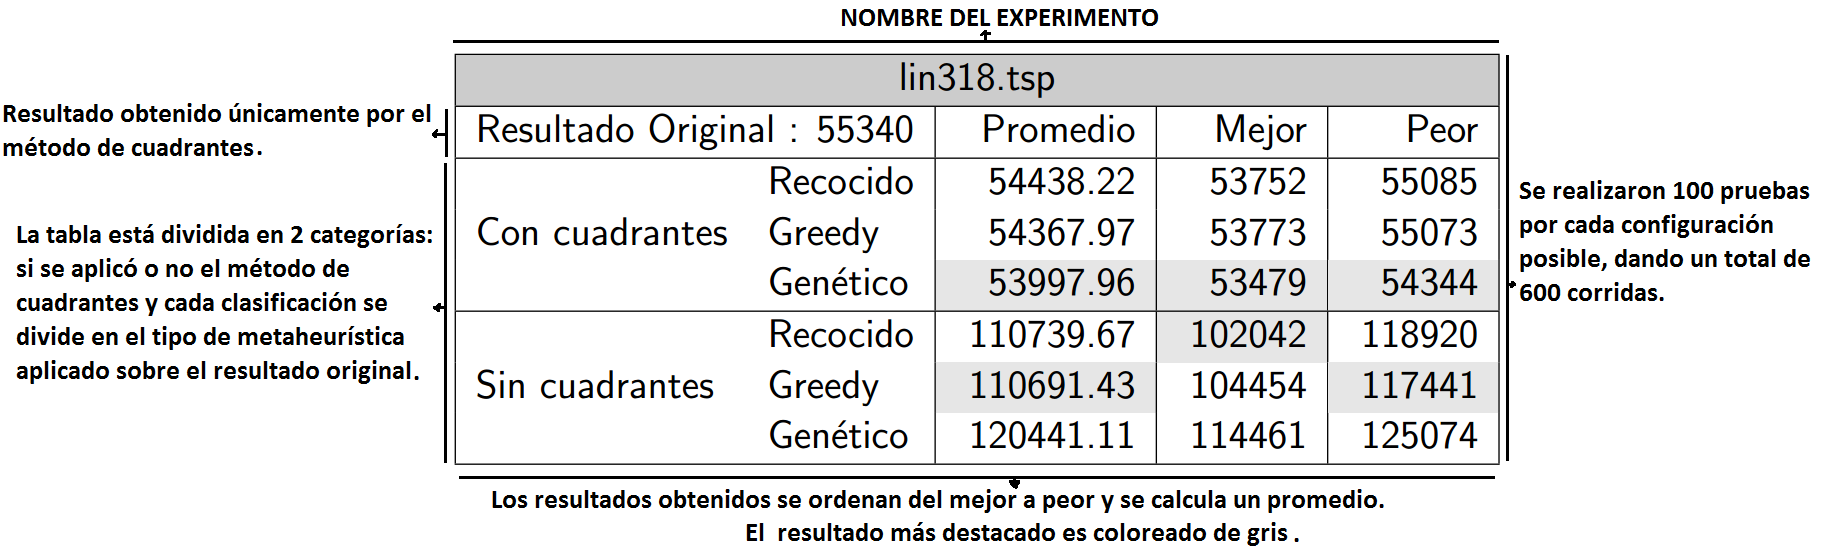
\includegraphics[width=1\textwidth]{PruebasResultados/Imagenes/ExplicacionExperimento_A.png}
        \caption{Explicación del experimento (punto A), tabla comparativa.}
        \label{fig:ExplicacionExperimento_A.png}
\end{figure}

\begin{figure}[hbtp]
    \centering
        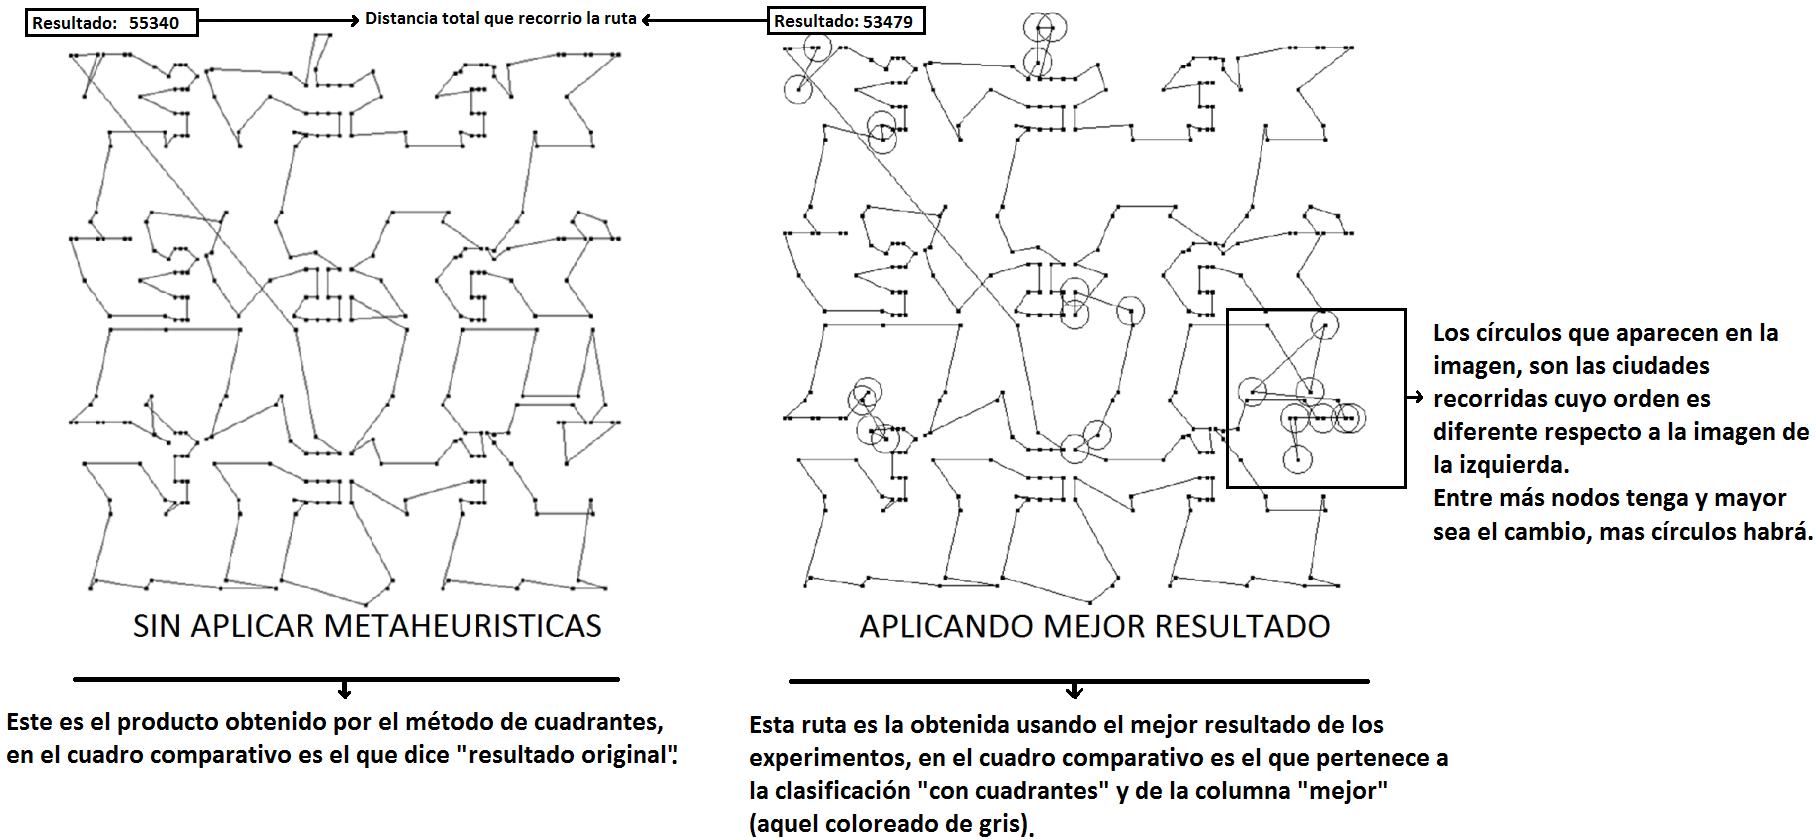
\includegraphics[width=1\textwidth]{PruebasResultados/Imagenes/ExplicacionExperimento_B.png}
        \caption{Explicación del experimento (punto B), comparación de rutas.}
        \label{fig:ExplicacionExperimento_B.png}
\end{figure}

\begin{figure}[hbtp]
    \centering
        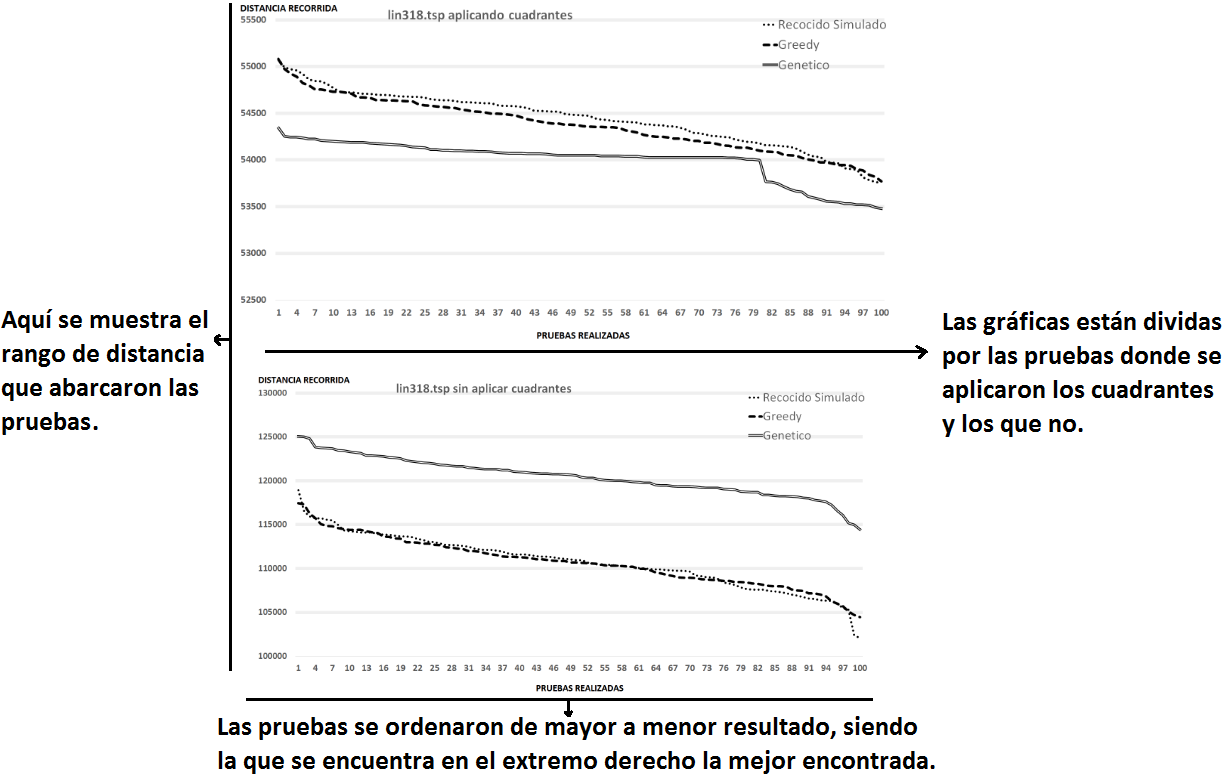
\includegraphics[width=1\textwidth]{PruebasResultados/Imagenes/ExplicacionExperimento_C.png}
        \caption{Explicación del experimento (punto C), gráfica que compara los resultados obtenidos aplicando o no el método de cuadrantes.}
        \label{fig:ExplicacionExperimento_C.png}
\end{figure}

\clearpage \newpage